\chapter{Specifikacija programske potpore}
		
	\section{Funkcionalni zahtjevi}
			

			\noindent \textbf{Dionici:}
			
			\begin{packed_enum}
				
				\item Pacijent
				\item Zaposlenik (medicinsko osoblje)				
				\item Administrator
                \item Razvojni tim:
                    \begin{packed_item}
                        \item Dora Kašik (voditelj)
                        \item Josip Begić
                        \item Erik Greblo
                        \item Anton Vivoda
                        \item Roko Krstičević
                        \item Katarina Mikulić
                        \item Marko Miletić
                    \end{packed_item}
				
			\end{packed_enum}
			
			\noindent \textbf{Aktori i njihovi funkcionalni zahtjevi:}
			
			
			\begin{packed_enum}
				\item  \underbar{Pacijent (inicijator) može:}
				
				\begin{packed_enum}
					
					\item Predati zahtjev za terapijom i dodjelom termina iste
                        \begin{packed_enum}
						
						\item  Ako dolazi na ponovljenu terapiju, u zahtjevu prilaže referencu na prethodno obavljenu terapiju
				
					\end{packed_enum}
					\item Izvršiti registraciju u sustav
					
					
				\end{packed_enum}
			
				\item  \underbar{Administrator (inicijator) može:}
				
				\begin{packed_enum}
					
					\item Upravljati  podacima o pacijentima i djelatnicima
					\item Upravljati podacima o dostupnoj opremi i prostorijama klinike
                    \item Vršiti postupke za zaštitu podataka
                    \item Dodavati nove djelatnike
     
				\end{packed_enum}

            \item  \underbar{Superadministrator (inicijator) može:}

                \begin{packed_enum}
					
					\item Dodijeliti djelatniku administratorskih ovlasti
					\item Ukloniti administratorske ovlasti djelatnika
                    \item Verificirati registraciju korisnika
                    \item Upravljati  podacima o pacijentima i djelatnicima
                    \item Upravljati podacima o dostupnoj opremi i prostorijama klinike
                    \item Vršiti postupke za zaštitu podataka
                    \item Dodavati nove djelatnike
     
				\end{packed_enum}

            \item  \underbar{Zaposlenik (inicijator) može:}
				
				\begin{packed_enum}
					
					\item Dodijeliti termin pacijentu
                        \begin{packed_enum}
						
						\item Nakon dodjele termina šalje pacijentu potrebne podatke o terminu putem elektroničke pošte
				
					\end{packed_enum}
					\item Pristupiti pregledu aktivnih prijava pacijenata
                    \item Pristupiti podatku o dostupnim djelatnicima
                    \item Pristupiti podatku o trajanju pojedinog zahvata
                    \item Pristupiti podacima o dostupnoj opremi i prostorijama klinike
                    \item Registrirati dolazak pacijenta na terapiju i rezultate nakon obavljene terapije
                    \item Prihvatiti ili odbiti zahtjev pacijenta za terminom terapije
					
					
				\end{packed_enum}

            \item  \underbar{Baza podataka (sudionik) može:}
				
				\begin{packed_enum}
					
					\item Pohranjuje podatke o korisnicima i njihovim ovlastima
					\item Pohranjuje podatke o terapijama
                    \item Pohranjuje podatke o čestim pitanjima
                    \item Pohranjuje podatke o prostorijama i opremi
     
				\end{packed_enum}
            
			\end{packed_enum}
			
			\eject 
			
			
				
			\subsection{Obrasci uporabe}
				
				
				\subsubsection{Opis obrazaca uporabe}
					

					\noindent \underbar{\textbf{UC1 - Registracija pacijenta}}
					\begin{packed_item}
	
						\item \textbf{Glavni sudionik: }Pacijent
						\item  \textbf{Cilj:} Registracija novog pacijenta u sustavu
						\item  \textbf{Sudionici:} Baza podataka/Sustav
						\item  \textbf{Preduvjet:} Bolesnik nema prethodno registriran račun
						\item  \textbf{Opis osnovnog tijeka:}
						
						\item[] \begin{packed_enum}
	
							\item Pacijent unosi osobne podatke, adresu elektroničke pošte i lozinku.
							\item Sustav provjerava ispravnost podataka.
							\item Sustav pohranjuje podatke i stvara korisnički račun.
	
						\end{packed_enum}
						
						\item  \textbf{Opis mogućih odstupanja:} Ako podaci nisu ispravni, sustav obavještava korisnika o potrebnim ispravkama.
						
						
					\end{packed_item}

                    \noindent \underbar{\textbf{UC2 - Prijava pacijenta}}
					\begin{packed_item}
	
						\item \textbf{Glavni sudionik: }Pacijent
						\item  \textbf{Cilj:} Pristup stranici rehabilitacije nakon prijave
						\item  \textbf{Sudionici:} Baza podataka
						\item  \textbf{Preduvjet:} Pacijent je registriran i prijavljen u sustav
						\item  \textbf{Opis osnovnog tijeka:}
						
						\item[] \begin{packed_enum}
	
							\item Pacijent šalje zahtjev za prijavom na sustav s korisničkim imenom i lozinkom.
							\item Sustav provjerava ispravnost podataka.
							\item Ako su podaci ispravni, pacijent je prijavljen u sustav.
	
						\end{packed_enum}
						
						\item  \textbf{Opis mogućih odstupanja:} Ako podaci nisu ispravni, sustav obavještava korisnika o potrebnim ispravkama. Ako pacijent nije registriran, sustav obavještava korisnika da nema važeći račun. 
						
						
					\end{packed_item}

                \noindent \underbar{\textbf{UC3 - Zahtjev za resetiranje lozinke}}
					\begin{packed_item}
	
						\item \textbf{Glavni sudionik: }Pacijent
						\item  \textbf{Cilj:} Prijava u sustav kako bi pristupio stranici rehabilitacije
						\item  \textbf{Sudionici:} Baza podataka/Sustav
						\item  \textbf{Preduvjet:} Korisnik ima registriran račun u sustavu
						\item  \textbf{Opis osnovnog tijeka:}
						
						\item[] \begin{packed_enum}
	
							\item Pacijent šalje zahtjev za poveznicu za resetiranje lozinke
							\item Sustav šalje poveznicu za resetiranje lozinke na korisnikovu adresu elektroničke pošte.
	
						\end{packed_enum}
						
						\item  \textbf{Opis mogućih odstupanja:} Ako se ne može pronaći korisnik s unesenom adresom e-pošte, sustav obavještava korisnika o neuspjelom zahtjevu. 
						
						
					\end{packed_item}

                \noindent \underbar{\textbf{UC4 - Spremanje nove lozinke}}
					\begin{packed_item}
	
						\item \textbf{Glavni sudionik: }Pacijent
						\item  \textbf{Cilj:} Spremiti novu lozinku nakon poveznice za resetiranje lozinke
						\item  \textbf{Sudionici:} Baza podataka/Sustav
						\item  \textbf{Preduvjet:} Korisnik je primio poveznicu za resetiranje lozinke i želi postaviti novu lozinku
						\item  \textbf{Opis osnovnog tijeka:}
						
						\item[] \begin{packed_enum}
	
							\item Pacijent šalje novu lozinku putem poveznice za resetiranje lozinke.
							\item Sustav sprema novu lozinku za korisnički račun.
	
						\end{packed_enum}
						
						\item  \textbf{Opis mogućih odstupanja:} Ako poveznica za resetiranje lozinke nije ispravna ili je istekla, sustav obavještava korisnika o neuspjelom ažuriranju lozinke. 
						
						
					\end{packed_item}

                \noindent \underbar{\textbf{UC5 - Dodavanje zaposlenika u bazu}}
					\begin{packed_item}
	
						\item \textbf{Glavni sudionik: }Administrator
						\item  \textbf{Cilj:} Registrirati novog zaposlenika u sustavu
						\item  \textbf{Sudionici:} Baza podataka/Sustav
						\item  \textbf{Preduvjet:} Korisnik ima administratorske ovlasti i prijavljen je u sustav
						\item  \textbf{Opis osnovnog tijeka:}
						
						\item[] \begin{packed_enum}
	
							\item Administrator šalje zahtjev za registraciju zaposleniika s podacima o zaposleniku.
							\item Sustav provjerava ispravnost podataka.
                            \item Sustav registrira zaposlenika u sustavu.
	
						\end{packed_enum}
						
						\item  \textbf{Opis mogućih odstupanja:} Ako podaci nisu ispravni, sustav obavještava administratora o potrebnim ispravkama.
						
						
					\end{packed_item}

                \noindent \underbar{\textbf{UC6 - Brisanje zaposlenika}}
					\begin{packed_item}
	
						\item \textbf{Glavni sudionik: }Administrator
						\item  \textbf{Cilj:} Deaktivirati račun određenog zaposlenika u sustav
						\item  \textbf{Sudionici:} Baza podataka/Sustav
						\item  \textbf{Preduvjet:} Korisnik ima administratorske ovlasti i prijavljen je u sustav
						\item  \textbf{Opis osnovnog tijeka:}
						
						\item[] \begin{packed_enum}
	
							\item Administrator šalje zahtjev za brisanje zaposlenika s određenim identifikatorom.
							\item Sustav označava zaposlenika kao neaktivnog u bazi podataka.
	
						\end{packed_enum}
						
						
					\end{packed_item}

                \noindent \underbar{\textbf{UC7 - Dodavanje učestalih pitanja (FAQ)}}
					\begin{packed_item}
	
						\item \textbf{Glavni sudionik: }Administrator
						\item  \textbf{Cilj:} Dodati novi FAQ u sustav
						\item  \textbf{Sudionici:} Baza podataka/Sustav
						\item  \textbf{Preduvjet:} Korisnik ima administratorske ovlasti i prijavljen je u sustav
						\item  \textbf{Opis osnovnog tijeka:}
						
						\item[] \begin{packed_enum}
	
							\item Administrator šalje zahtjev za dodavanje novog FAQ-a s podacima o FAQ-u.
							\item Sustav provjerava ispravnost podataka.
                            \item Sustav dodaje novi FAQ u sustav.
	
						\end{packed_enum}
						
						\item  \textbf{Opis mogućih odstupanja:} Ako podaci nisu ispravni, sustav obavještava administratora o potrebnim ispravkama.
						
						
					\end{packed_item}

                \noindent \underbar{\textbf{UC8 - Prikaz svih učestalih pitanja (FAQ-a)}}
					\begin{packed_item}
	
						\item \textbf{Glavni sudionik: }Bilo koji korisnik
						\item  \textbf{Cilj:} Prikazati popis svih FAQ-ova u sustavu
						\item  \textbf{Sudionici:} Baza podataka/Sustav
						\item  \textbf{Opis osnovnog tijeka:}
						
						\item[] \begin{packed_enum}
	
							\item Korisnik šalje zahtjev za dohvaćanje svih FAQ-ova.
							\item Sustav dohvaća popis FAQ-ova iz baze podataka.
                            \item Sustav vraća odgovor s popisom FAQ-ova.
	
						\end{packed_enum}
						
						
					\end{packed_item}

                \noindent \underbar{\textbf{UC9 - Brisanje učestalih pitanja (FAQ)}}
					\begin{packed_item}
	
						\item \textbf{Glavni sudionik: }Administrator
						\item  \textbf{Cilj:} Brisati određeni FAQ iz sustava
						\item  \textbf{Sudionici:} Baza podataka/Sustav
						\item  \textbf{Preduvjet:} Korisnik ima administratorske ovlasti i prijavljen je u sustav
						\item  \textbf{Opis osnovnog tijeka:}
						
						\item[] \begin{packed_enum}
	
							\item Administrator šalje zahtjev za brisanje FAQ-a s određenim identifikatorom.
							\item Sustav označava FAQ kao neaktivan u bazi podataka.
	
						\end{packed_enum}

						
					\end{packed_item}

                \noindent \underbar{\textbf{UC10 - Kreiranje sobe}}
					\begin{packed_item}
	
						\item \textbf{Glavni sudionik: }Zaposlenik
						\item  \textbf{Cilj:} Kreirati novu sobu u sustavu
						\item  \textbf{Sudionici:} Baza podataka/Sustav
						\item  \textbf{Preduvjet:} Korisnik ima administratorske ovlasti i prijavljen je u sustav
						\item  \textbf{Opis osnovnog tijeka:}
						
						\item[] \begin{packed_enum}
	
							\item Zaposlenik šalje zahtjev za kreiranje nove sobe s potrebnim podacima.
							\item Sustav provjerava ispravnost podataka.
	
						\end{packed_enum}
						
						\item  \textbf{Opis mogućih odstupanja:} Ako podaci nisu ispravni, sustav obavještava administratora o potrebnim ispravkama.
						
						
					\end{packed_item}

                \noindent \underbar{\textbf{UC11 - Pregled svih soba}}
					\begin{packed_item}
	
						\item \textbf{Glavni sudionik: }Zaposlenik
						\item  \textbf{Cilj:} Prikazati sve sobe u sustavu
						\item  \textbf{Sudionici:} Baza podataka/Sustav
						\item  \textbf{Preduvjet:} Korisnik ima administratorske ovlasti i prijavljen je u sustav
						\item  \textbf{Opis osnovnog tijeka:}
						
						\item[] \begin{packed_enum}
	
							\item Zaposlenik šalje zahtjev za dohvaćanje svih soba.
							\item Sustav dohvaća sve sobe iz baze podataka.
                            \item Sustav vraća odgovor s popisom soba.
	
						\end{packed_enum}
						
						
					\end{packed_item}

                \noindent \underbar{\textbf{UC12 - Pregled sobe po identifikacijskom broju}}
					\begin{packed_item}
	
						\item \textbf{Glavni sudionik: }Zaposlenik
						\item  \textbf{Cilj:} Pregledati pojedinu sobu u sustavu
						\item  \textbf{Sudionici:} Baza podataka/Sustav
						\item  \textbf{Preduvjet:} Korisnik ima administratorske ovlasti i prijavljen je u sustav
						\item  \textbf{Opis osnovnog tijeka:}
						
						\item[] \begin{packed_enum}
	
							\item Zaposlenik šalje zahtjev za dohvat sobe  s određenim identifikatorom.
							\item Sustav provjerava postoji li soba s navedenim identifikacijskim brojem.
                            \item Ako postoji, sustav prikazuje podatke o sobi.
	
						\end{packed_enum}
						
						\item  \textbf{Opis mogućih odstupanja:} Ako soba s navedenim identifikacijskim brojem ne postoji, sustav obavještava zaposlenika.
						
						
					\end{packed_item}

                \noindent \underbar{\textbf{UC13 - Brisanje sobe}}
					\begin{packed_item}
	
						\item \textbf{Glavni sudionik: }Zaposlenik
						\item  \textbf{Cilj:} Obrisati sobu iz sustava
						\item  \textbf{Sudionici:} Baza podataka/Sustav
						\item  \textbf{Preduvjet:} Korisnik ima administratorske ovlasti i prijavljen je u sustav
						\item  \textbf{Opis osnovnog tijeka:}
						
						\item[] \begin{packed_enum}
	
							\item Zaposlenik šalje zahtjev za brisanje sobe s određenim identifikacijskim brojem.
							\item Sustav provjerava postoji li soba s navedenim identifikacijskim brojem.
                            \item Ako postoji, sustav briše sobu.
	
						\end{packed_enum}
						
						\item  \textbf{Opis mogućih odstupanja:} Ako podaci nisu ispravni, sustav obavještava administratora o potrebnim ispravkama.
						
						
					\end{packed_item}

                \noindent \underbar{\textbf{UC14 - Kreiranje opreme}}
					\begin{packed_item}
	
						\item \textbf{Glavni sudionik: }Zaposlenik
						\item  \textbf{Cilj:} Kreirati novu opremu u sustavu
						\item  \textbf{Sudionici:} Baza podataka/Sustav
						\item  \textbf{Preduvjet:} Korisnik ima administratorske ovlasti i prijavljen je u sustav
						\item  \textbf{Opis osnovnog tijeka:}
						
						\item[] \begin{packed_enum}
	
							\item Korisnik šalje zahtjev za kreiranje nove opreme s potrebnim podacima.
							\item Sustav provjerava ispravnost podataka.
                            \item Sustav kreira novu opremu u sustav.
	
						\end{packed_enum}
						
						\item  \textbf{Opis mogućih odstupanja:} Ako podaci nisu ispravni, sustav obavještava zaposlenika o potrebnim ispravkama.
						
						
					\end{packed_item}

                \noindent \underbar{\textbf{UC15 - Pregled svih oprema}}
					\begin{packed_item}
	
						\item \textbf{Glavni sudionik: }Zaposlenik
						\item  \textbf{Cilj:} Prikazati sve sobe u sustavu
						\item  \textbf{Sudionici:} Baza podataka/Sustav
						\item  \textbf{Preduvjet:} Korisnik ima administratorske ovlasti i prijavljen je u sustav
						\item  \textbf{Opis osnovnog tijeka:}
						
						\item[] \begin{packed_enum}
	
							\item Zaposlenik šalje zahtjev za dohvaćanje svih oprema.
							\item Sustav dohvaća svu opremu iz baze podataka.
                            \item Sustav vraća odgovor s popisom opreme.
	
						\end{packed_enum}
						
					\end{packed_item}

                \noindent \underbar{\textbf{UC16 - Pregled opreme po identifikacijskom broju}}
					\begin{packed_item}
	
						\item \textbf{Glavni sudionik: }Zaposlenik
						\item  \textbf{Cilj:} Pregledati pojedinu opremu u sustavu
						\item  \textbf{Sudionici:} Baza podataka/Sustav
						\item  \textbf{Preduvjet:} Korisnik ima administratorske ovlasti i prijavljen je u sustav
						\item  \textbf{Opis osnovnog tijeka:}
						
						\item[] \begin{packed_enum}
	
							\item Zaposlenik šalje zahtjev za dohvat opreme s određenim identifikatorom.
							\item Sustav provjerava postoji li oprema s navedenim identifikacijskim brojem.
                            \item Ako postoji, sustav prikazuje podatke o opremi.
	
						\end{packed_enum}
						
						\item  \textbf{Opis mogućih odstupanja:} Ako oprema s navedenim identifikacijskim brojem ne postoji, sustav obavještava zaposlenika.
						
						
					\end{packed_item}

                \noindent \underbar{\textbf{UC17 - Brisanje opreme}}
					\begin{packed_item}
	
						\item \textbf{Glavni sudionik: }Zaposlenik
						\item  \textbf{Cilj:} Obrisati opremu iz sustava
						\item  \textbf{Sudionici:} Baza podataka/Sustav
						\item  \textbf{Preduvjet:} Korisnik ima administratorske ovlasti i prijavljen je u sustav
						\item  \textbf{Opis osnovnog tijeka:}
						
						\item[] \begin{packed_enum}
	
							\item Zaposlenik šalje zahtjev za brisanje opreme s određenim identifikacijskim brojem.
							\item Sustav sustav provjerava postoji li oprema s navedenim identifikacijskim brojem.
                            \item Ako postoji, sustav briše opremu.
	
						\end{packed_enum}
						
						
					\end{packed_item}

                \noindent \underbar{\textbf{UC18 - Prikaz svih pacijenata}}
					\begin{packed_item}
	
						\item \textbf{Glavni sudionik: }Administrator
						\item  \textbf{Cilj:} Prikazati popis svih pacijenata u sustavu
						\item  \textbf{Sudionici:} Baza podataka/Sustav
						\item  \textbf{Preduvjet:} Korisnik ima administratorske ovlasti i prijavljen je u sustav
						\item  \textbf{Opis osnovnog tijeka:}
						
						\item[] \begin{packed_enum}
	
							\item Administrator šalje zahtjev za dohvaćanje svih pacijenata.
							\item Sustav dohvaća popis pacijenata iz baze podataka.
                            \item Sustav vraća odgovor s popisom pacijenata.
	
						\end{packed_enum}
						
						
					\end{packed_item}

                \noindent \underbar{\textbf{UC19 - Deaktivacija pacijentovog računa}}
					\begin{packed_item}
	
						\item \textbf{Glavni sudionik: }Pacijent, Zaposlenik, Admin
						\item  \textbf{Cilj:} Deaktivirati račun određenog pacijenta u sustavu
						\item  \textbf{Sudionici:} Baza podataka/Sustav
						\item  \textbf{Preduvjet:} Korisnik je prijavljen u sustav
						\item  \textbf{Opis osnovnog tijeka:}
						
						\item[] \begin{packed_enum}
	
							\item Korisnik šalje zahtjev za deaktivaciju pacijentovog računa s određenim identifikatorom.
							\item Sustav označava pacijenta kao neaktivnog u bazi podataka.
	
						\end{packed_enum}
						
						
					\end{packed_item}

                \noindent \underbar{\textbf{UC20 - Kreiranje terapije za pacijenta}}
					\begin{packed_item}
	
						\item \textbf{Glavni sudionik: }Pacijent, Zaposlenik
						\item  \textbf{Cilj:} Dodati novu terapiju za određenog pacijenta
						\item  \textbf{Sudionici:} Baza podataka/Sustav
						\item  \textbf{Preduvjet:} Korisnik je prijavljen u sustav
						\item  \textbf{Opis osnovnog tijeka:}
						
						\item[] \begin{packed_enum}
	
							\item Korisnik šalje zahtjev za dodavanje nove terapije s podacima o terapiji.
							\item Sustav provjerava ispravnost podataka.
                            \item Sustav dodaje novu terapiju za određenog pacijenta u sustavu.
	
						\end{packed_enum}
						
						\item  \textbf{Opis mogućih odstupanja:} Ako podaci nisu ispravni, sustav obavještava korisnika o potrebnim ispravkama.
						
						
					\end{packed_item}

                \noindent \underbar{\textbf{UC21 - Prikaz svih terapija za pacijenta}}
					\begin{packed_item}
	
						\item \textbf{Glavni sudionik: }Pacijent
						\item  \textbf{Cilj:} Prikazati popis svih terapija za određenog pacijenta
						\item  \textbf{Sudionici:} Baza podataka/Sustav
						\item  \textbf{Preduvjet:} Korisnik je prijavljen u sustav
						\item  \textbf{Opis osnovnog tijeka:}
						
						\item[] \begin{packed_enum}
	
							\item Korisnik šalje zahtjev za dohvaćanje svih terapija za određenog pacijenta.
							\item Sustav dohvaća popis terapija iz baze podataka za određenog pacijenta.
                            \item Sustav vraća odgovor s popisom terapija.
	
						\end{packed_enum}
						
						
					\end{packed_item}

                \noindent \underbar{\textbf{UC22 - Unos rezultata terapije}}
					\begin{packed_item}
	
						\item \textbf{Glavni sudionik: }Zaposlenik
						\item  \textbf{Cilj:} Unijeti rezultate terapije u sustav
						\item  \textbf{Sudionici:} Baza podataka/Sustav
						\item  \textbf{Preduvjet:} Korisnik ima ovlasti zaposlenika i prijavljen je u sustav
						\item  \textbf{Opis osnovnog tijeka:}
						
						\item[] \begin{packed_enum}
	
							\item Zaposlenik šalje zahtjev za unos rezultata terapije s podacima o rezultatima.
							\item Sustav provjerava ispravnost podataka.
                            \item Sustav unosi rezultate terapije u sustav.
	
						\end{packed_enum}
						
						\item  \textbf{Opis mogućih odstupanja:} Ako podaci nisu ispravni, sustav obavještava zaposlenika o potrebnim ispravkama.
						
						
					\end{packed_item}

                \noindent \underbar{\textbf{UC23 - Dodjela administratorskih ovlasti}}
					\begin{packed_item}
	
						\item \textbf{Glavni sudionik: }Superadministrator
						\item  \textbf{Cilj:} Dodjela administratorskih ovlasti radi lakšeg upravljanja sustavom
						\item  \textbf{Sudionici:} Baza podataka/Sustav
						\item  \textbf{Preduvjet:} Korisnik ima ovlasti superadministratora i prijavljen je u sustav
						\item  \textbf{Opis osnovnog tijeka:}
						
						\item[] \begin{packed_enum}
	
							\item Superadministator šalje zahtjev za dodjelu administratorskih ovlasti određenom korisniku.
							\item Sustav provjerava ispravnost zahtjeva i potvrđuje administratorske ovlasti korisniku.
                            \item Sustav ažurira informacije o ovlastima korisnika u bazi podataka.
	
						\end{packed_enum}
						
						\item  \textbf{Opis mogućih odstupanja:} Ako podaci nisu ispravni ili korisnik već ima administratorske ovlasti, sustav obavještava superadministratora o potrebnim ispravkama ili prekoračenju ovlasti.
						
						
					\end{packed_item}

                \noindent \underbar{\textbf{UC24 - Uklanjanje administratorskih ovlasti}}
					\begin{packed_item}
	
						\item \textbf{Glavni sudionik: }Superadministrator
						\item  \textbf{Cilj:} Uklanjanje administratorskih ovlasti korisniku u sustavu
						\item  \textbf{Sudionici:} Baza podataka/Sustav
						\item  \textbf{Preduvjet:} Korisnik ima ovlasti superadministratora i prijavljen je u sustav
						\item  \textbf{Opis osnovnog tijeka:}
						
						\item[] \begin{packed_enum}
	
							\item Administrator šalje zahtjev za uklanjanje administratorskih ovlasti određenom korisniku.
							\item Sustav provjerava ispravnost zahtjeva i uklanja administratorske ovlasti korisniku.
                            \item Sustav ažurira informacije o ovlastima korisnika u bazi podataka.
	
						\end{packed_enum}
						
						\item  \textbf{Opis mogućih odstupanja:} Ako podaci nisu ispravni ili korisnik nema administratorske ovlasti, sustav obavještava administratora o potrebnim ispravkama ili nedostatku ovlasti za uklanjanje.
						
						
					\end{packed_item}

                \noindent \underbar{\textbf{UC25 - Prikaz svih zaposlenika}}
					\begin{packed_item}
	
						\item \textbf{Glavni sudionik: }Administrator
						\item  \textbf{Cilj:} Prikazati popis svih zaposlenika u sustavu
						\item  \textbf{Sudionici:} Baza podataka/Sustav
						\item  \textbf{Preduvjet:} Korisnik ima administratorske ovlasti i prijavljen je u sustav
						\item  \textbf{Opis osnovnog tijeka:}
						
						\item[] \begin{packed_enum}
	
							\item Administrator šalje zahtjev za dohvaćanje svih djelatnika.
							\item Sustav dohvaća popis zaposlenika iz baze podataka.
                            \item Sustav vraća odgovor s popisom zaposlenika.
	
						\end{packed_enum}
						
						
					\end{packed_item}
     
				\subsubsection{Dijagrami obrazaca uporabe}
					
					\begin{figure}[H]
			         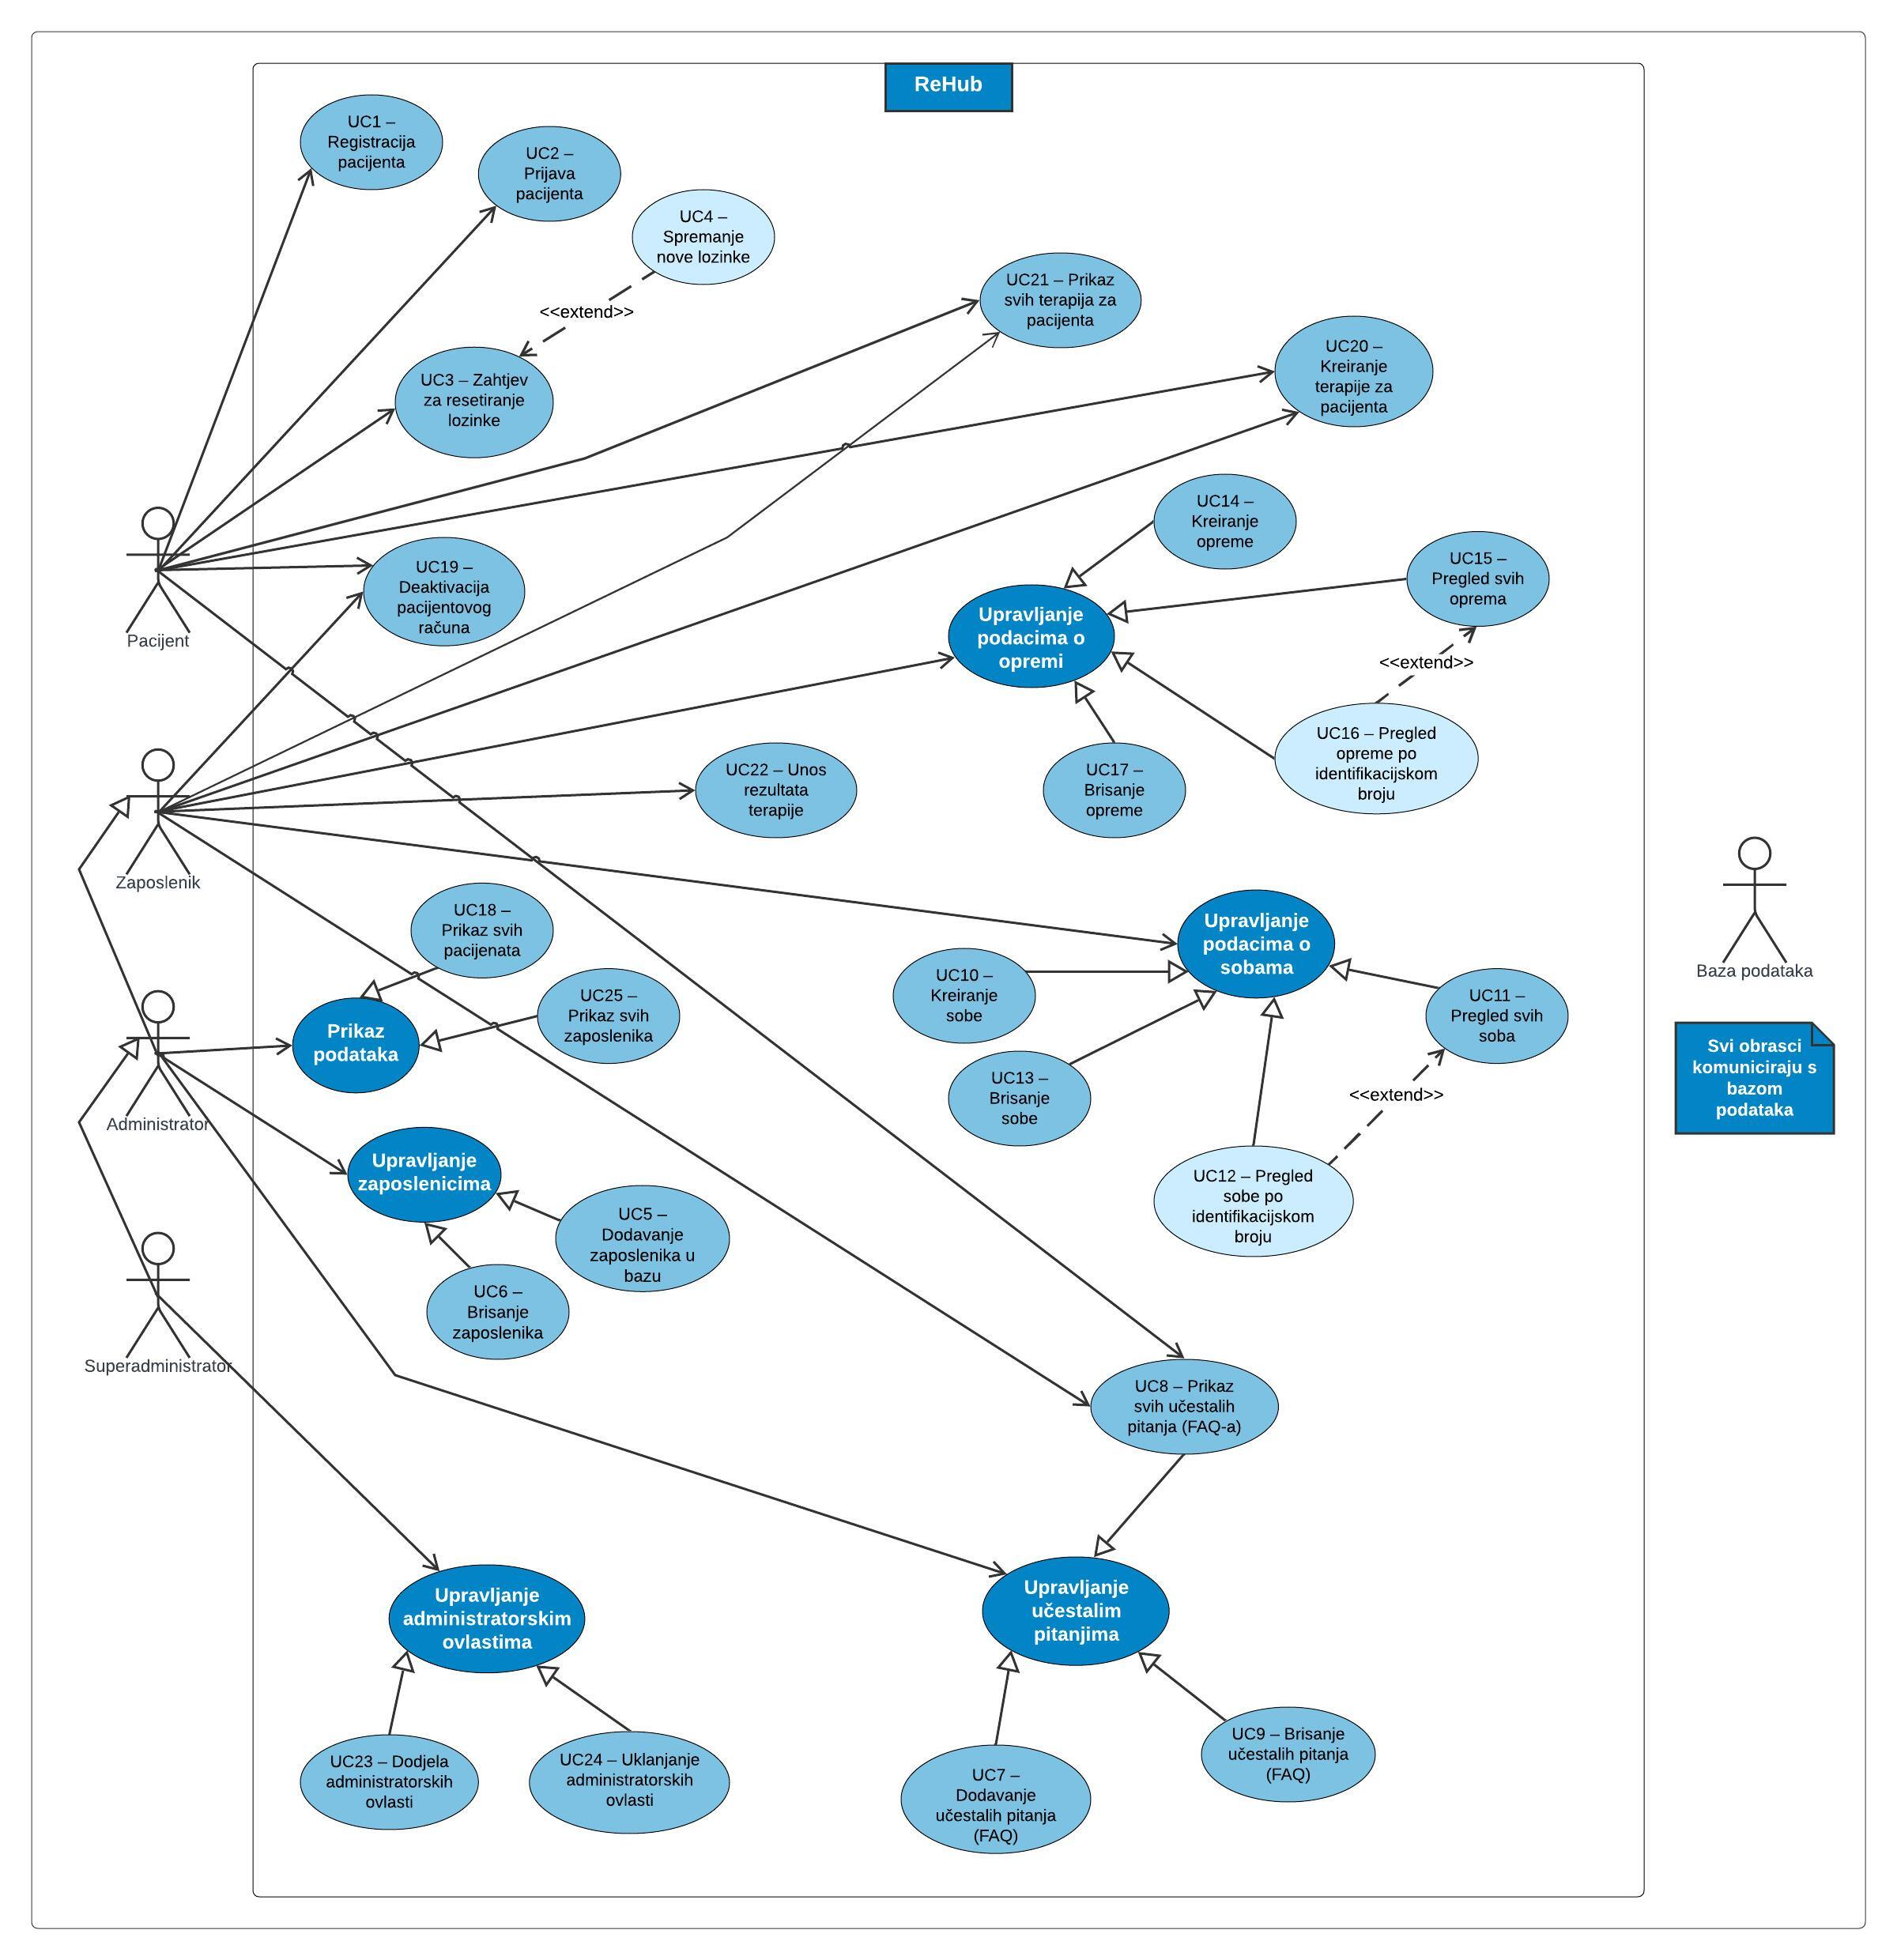
\includegraphics[scale=0.35]{dijagrami/ReHub Use case diagram.jpeg}
			         \centering
			         \caption{Dijagram obrazaca uporabe}
			         \label{fig:UseCaseDiagram}
		          \end{figure}
				\eject		
				
			\subsection{Sekvencijski dijagrami}
				
				U sljedećem dijelu prikazani su sekvencijski dijagrami i njihovi opisi.
                \subsubsection{Obrazac uporabe UC18 – Prikaz svih pacijenata i UC25 – Prikaz svih zaposlenika}

                    Korisnik odabire opciju "Prikaži sve pacijente" ili "Prikaži sve zaposlenike" unutar web-aplikacije. Web-aplikacija iz baze podataka dohvaća sve relevantne informacije o pacijentima odnosno zaposlenicima. Ako baza podataka vrati informacije o pacijentima, web-aplikacija ih prikazuje korisniku, omogućujući mu pregled detalja poput imena, adrese, kontakt informacija itd. U suprotnom, ispisuje poruku "Nema dostupnih pacijenata". Ako korisnik odabere opciju "Prikaži sve zaposlenike", web-aplikacija prikazuje informacije o svim zaposlenicima, uključujući njihova imena, pozicije, kontakt informacije itd. U suprotnom, ispisuje poruku "Nema dostupnih zaposlenika".

                \begin{figure}[H]
			         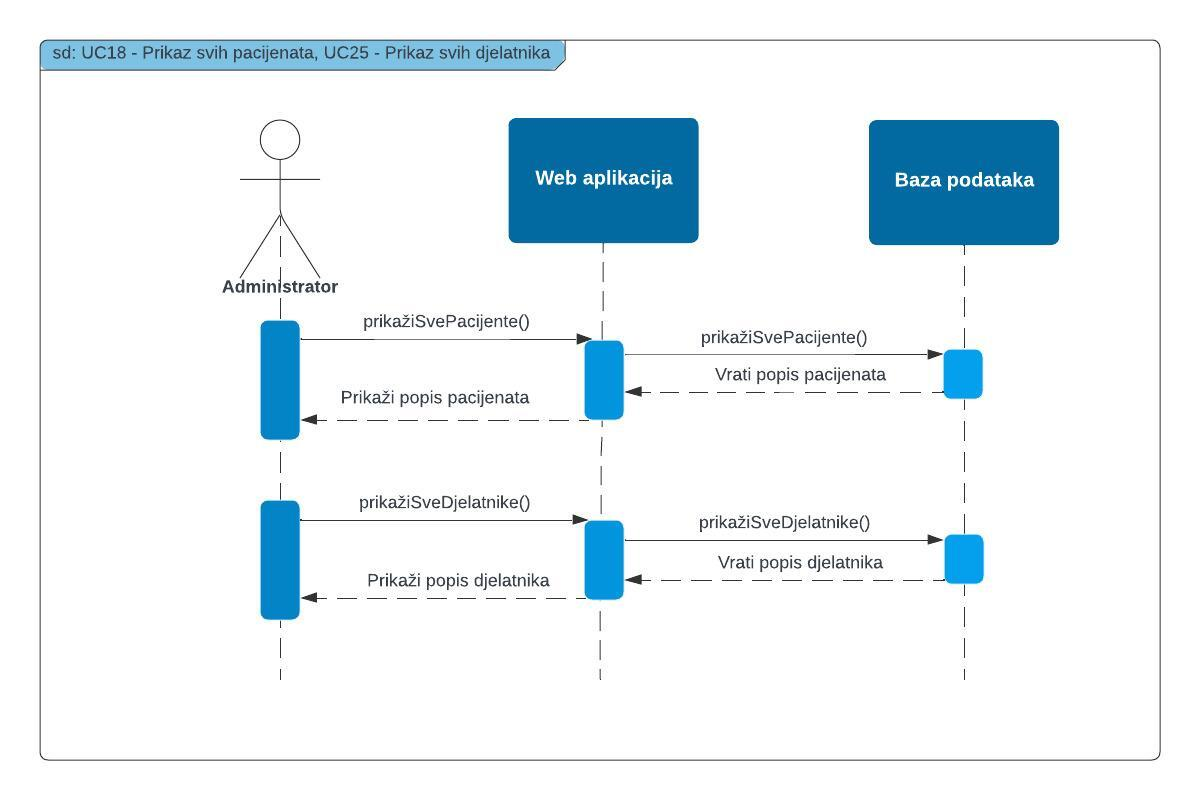
\includegraphics[scale=0.7]{dijagrami/Sequence diagram for ReHub admin.jpeg}
			         \centering
			         \caption{Sekvencijski dijagram za UC18/25}
			         \label{fig:SequenceDiagram1}
		        \end{figure}

                \eject

                \subsubsection{Obrazac uporabe UC8 – Prikaz svih učestalih pitanja, UC11 – Pregled svih soba i UC15 – Prikaz svih oprema}

                    Korisnik odabire opciju "Učestala pitanja" unutar web-aplikacije. Web-aplikacija iz baze podataka dohvaća sve učestala pitanja. Ako postoje učestala pitanja, aplikacija ih prikazuje korisniku, pružajući odgovore i relevantne informacije. Ako nema učestalih pitanja, ispisuje poruku "Nema dostupnih učestalih pitanja." Dodatna funkcionalnost: Korisnik ima mogućnost filtriranja pitanja po kategorijama ili ključnim riječima. Korisnik odabire opciju "Pregled svih soba" unutar web-aplikacije. Web-aplikacija iz baze podataka dohvaća sve informacije o sobama. Ako postoje sobe, aplikacija ih prikazuje korisniku s detaljima poput broja sobe, vrste, dostupnih sadržaja itd. Ako nema dostupnih soba, ispisuje poruku "Nema dostupnih soba." Dodatna funkcionalnost: Korisnik može filtrirati sobe prema vrsti, kapacitetu ili dostupnim sadržajima. Korisnik odabire opciju "Prikaz svih oprema" unutar web-aplikacije. Web-aplikacija iz baze podataka dohvaća informacije o svim dostupnim opremama. Ako postoje informacije o opremama, aplikacija ih prikazuje korisniku, pružajući detalje o vrstama opreme, količini dostupnih itd. Ako nema dostupnih informacija o opremama, ispisuje poruku "Nema dostupne opreme." Dodatna funkcionalnost: Korisnik može filtrirati opremu prema vrsti ili dostupnosti.

                    \begin{figure}[H]
			         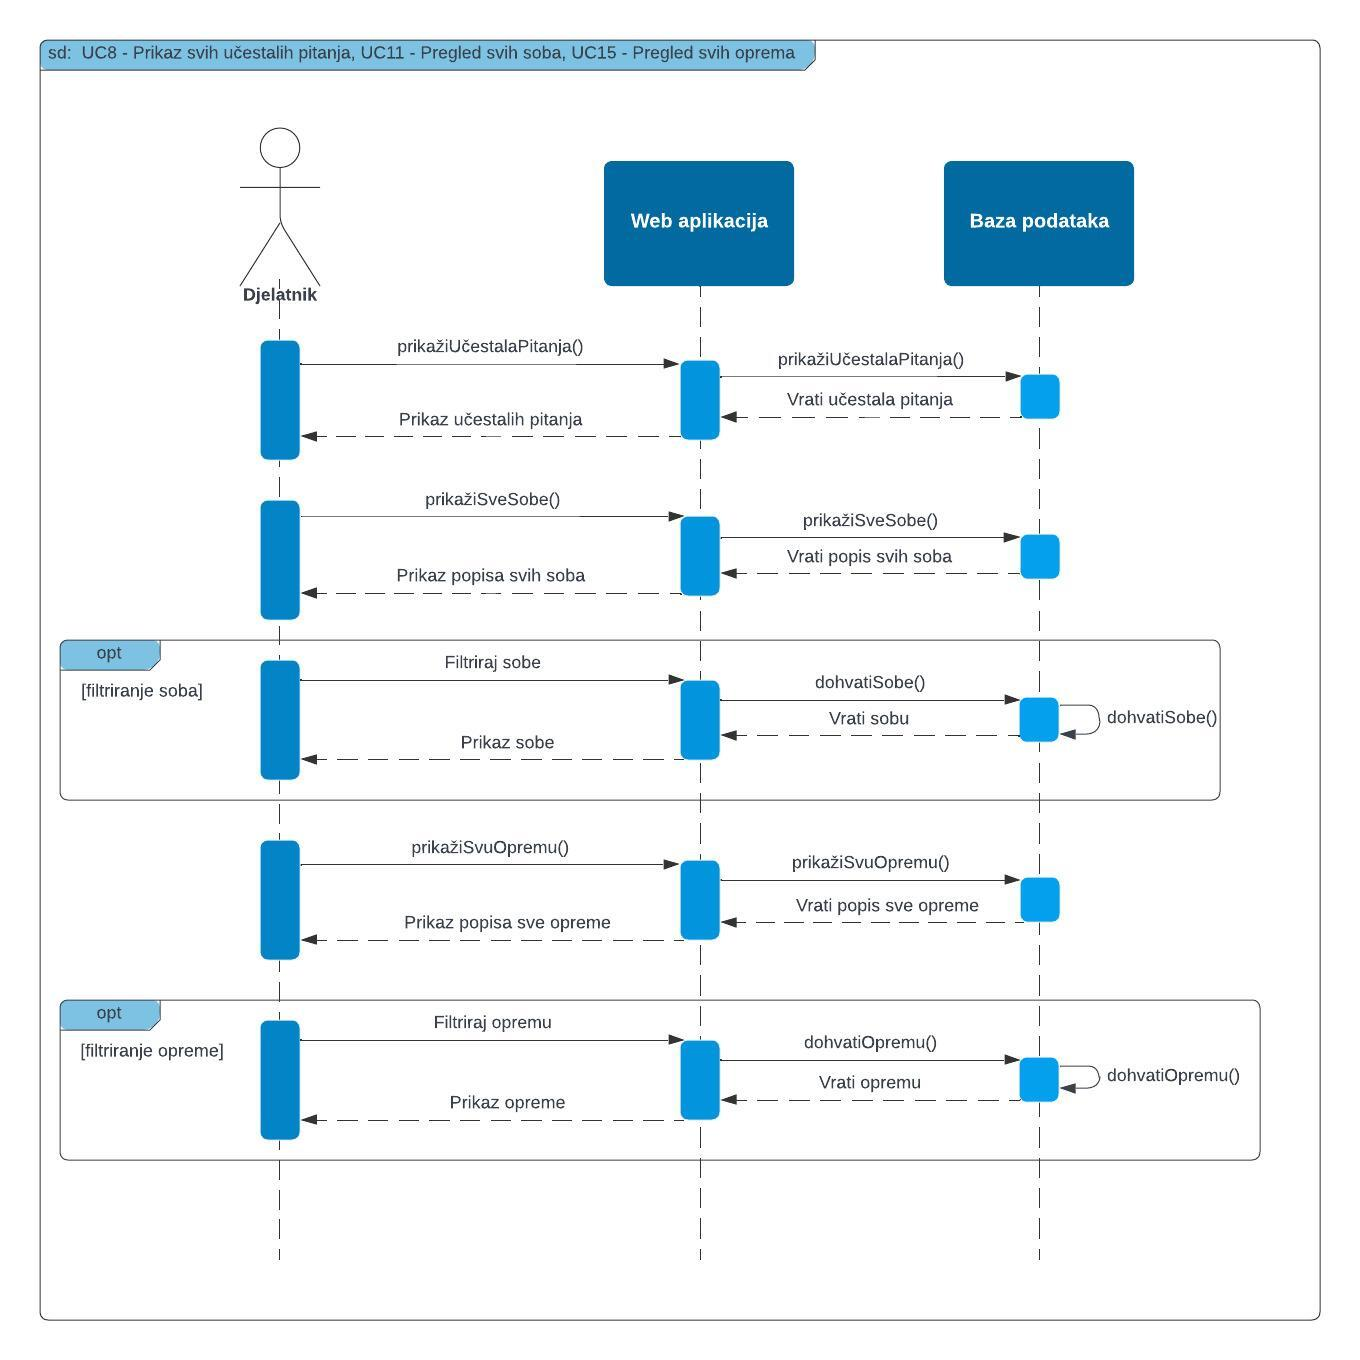
\includegraphics[scale=0.7]{dijagrami/Sequence diagram for ReHub.jpeg}
			         \centering
			         \caption{Sekvencijski dijagram za UC8/11/15}
			         \label{fig:SequenceDiagram2}
		          \end{figure}
                
				\eject
	
		\section{Ostali zahtjevi}
		 
			 \begin{packed_enum}
				
				\large \item Sustav mora podržavati više različitih uloga korisnika \normalsize
                    \begin{packed_item}
                        \item Sustav treba omogućiti definiranje različitih razina pristupa i funkcionalnosti ovisno o ulozi korisnika (Administrator, Liječnik, Pacijent, itd.).
                    \end{packed_item}
				 \large \item Korisnički podaci moraju biti sigurno pohranjeni u sustavu	\normalsize
                    \begin{packed_item}
                        \item Sustav treba koristiti kriptiranje za pohranu i prijenos osjetljivih korisničkih podataka kako bi osigurao privatnost i sigurnost informacija.
                    \end{packed_item}
				 \large \item Brza i pouzdana veza s bazom podataka \normalsize
                    \begin{packed_item}
                        \item Sustav treba osigurati pouzdanu vezu s bazom podataka kako bi pristup podacima bio brz i otporan na vanjske pogreške.
                    \end{packed_item}
                 \large \item Odgovarajuće vrijeme izvršavanja za upite prema bazi podataka \normalsize
                    \begin{packed_item}
                        \item Izvršavanje upita koji pristupaju bazi podataka ne smije trajati dulje od definiranog vremena, kako bi se osigurala učinkovitost sustava.
                    \end{packed_item}
                 \large \item Podrška za hrvatsku abecedu u korisničkom sučelju i pri unosu teksta \normalsize
                    \begin{packed_item}
                        \item Korisničko sučelje i sustav trebaju podržavati hrvatsku abecedu pri unosu, prikazu i obradi tekstualnih podataka.
                    \end{packed_item}
                 \large \item Web aplikacija implementirana korištenjem objektno-orijentiranih jezika \normalsize
                    \begin{packed_item}
                        \item Sustav treba biti implementiran kao web aplikacija koristeći suvremene objektno-orijentirane jezike kako bi bio skalabilan i održiv.
                    \end{packed_item}
                 \large \item Intuitivan i lagan za korištenje \normalsize
                    \begin{packed_item}
                        \item Korisničko sučelje treba biti intuitivno i jednostavno za korištenje kako bi korisnici mogli efikasno koristiti sustav bez potrebe za dodatnim uputama.
                    \end{packed_item}
                 \large \item Nadogradnja sustava bez narušavanja postojećih funkcionalnosti \normalsize
                    \begin{packed_item}
                        \item Nadogradnje sustava trebaju biti provedene bez negativnog utjecaja na postojeće funkcionalnosti kako bi korisnici nastavili neometano koristiti sustav.
                    \end{packed_item}
                 \large \item Zaštita od neispravnog korištenja korisničkog sučelja \normalsize
                    \begin{packed_item}
                        \item Neispravno korištenje korisničkog sučelja ne smije narušiti funkcionalnosti i rad sustava. Sustav treba biti otporan na potencijalne greške ili zloupotrebu od strane korisnika.
                    \end{packed_item}
                    
				
			\end{packed_enum}
			 
			 
			 
	